% !TeX root = RJwrapper.tex
\title{\pkg{DChaos}: An R Package for Chaotic Time Series Analysis}
\author{by Julio E. Sandubete and Lorenzo Escot}

\maketitle

\abstract{
Chaos theory has been hailed as a revolution of thoughts and attracting ever-increasing attention of many scientists from diverse disciplines. Chaotic systems are non-linear deterministic dynamic systems which can behave like an erratic and apparently random motion. A relevant field inside chaos theory is the detection of chaotic behavior from empirical time-series data. One of the main features of chaos is the well-known initial-value sensitivity property. Methods and techniques related to testing the hypothesis of chaos try to quantify the initial-value sensitive property estimating the so-called Lyapunov exponents. This paper describes the main estimation methods of the Lyapunov exponent from time series data. At the same time, we present the \pkg{DChaos} library. R users may compute the delayed-coordinate embedding vector from time series data, estimates the best-fitted neural net model from the delayed-coordinate embedding vectors, calculates analytically the partial derivatives from the chosen neural nets model. They can also obtain the neural net estimator of the Lyapunov exponent from the partial derivatives computed previously by two different procedures and four ways of subsampling by blocks. To sum up, the \pkg{DChaos} package allows the R users to test robustly the hypothesis of chaos in order to know if the data-generating process behind time series behaves chaotically or not. The package's functionality is illustrated by examples.}

%%%%%%%%%%%%%%%%%%%%%%%%%%%%%%%%
%%%%%%%%%% INTRODUCTION %%%%%%%%%%%%%
%%%%%%%%%%%%%%%%%%%%%%%%%%%%%%%%

\section{Introduction}

According to the literature, countless techniques have been developed and used to estimate the complexity of time series data; for a review see, e.g., \cite{Faggini:2014}, \cite{Bradley:2015}, \cite{Tang:2015}. We have focused on methods derived from chaos theory which estimates the complexity of a dataset through exploring the structure of the attractor. Particularly, we have been interested in the so-called \textit{Lyapunov exponent} ($\lambda$) as an attractor invariant measure. Quantifing chaos through this kind of quantitative measure is a key point for understanding chaotic behavior. Hence, our interest will be to test the hypothesis of chaos defined as follows:

\begin{equation}
\begin{array}{*{20}{c}}
  {{H_0}:{{\hat \lambda }_k} > 0} \\ 
  {{H_1}:{{\hat \lambda }_k} \leqslant 0},
\end{array}
\label{eq0}
\end{equation}

\noindent for $k = 1,2,3, \ldots$ on a $k$-dimensional system. Reject the null hypothesis ${H_0}:{{\hat \lambda }_k} > 0$ means lack of chaotic behavior. That is, the data-generating process does not have a chaotic attractor because it does not show the property of sensitivity to initial conditions, see \cite{Gencay1992}. The existence of a positive Lyapunov exponent makes it possible to distinguish whether an apparently erratic, non-cyclical, and aperiodic dynamic system is random or chaotic. In this sense, a positive Lyapunov exponent allows us to evidence that a deterministic generating system exists behind that chaotic system in spite of showing an apparently random dynamic behavior. This fact would provide us to take advantage of this deterministic character to be able to seek modeling of time series using non-linear dynamic models, make reliable predictions, at least within the limits established by the sensitivity to the initial conditions, and control over the variables of these chaotic deterministic dynamic systems, see \cite{Diaz2019}.

This ergodic measure can be defined as follows. Let ${{X_t}} = f\left( {X_{t - 1}} \right)$ be a difference equation where $f:{\mathbb{R}^{k}} \to {\mathbb{R}^{k}}$ for $t = 1,2,3, \ldots ,n$. For a $k$-dimensional system, there will be $k$ Lyapunov exponents which are given by

\begin{align}
{\lambda _k}\left( {{X_0}} \right) &= \mathop {\lim }\limits_{t \to \infty } \frac{1}{t}\left\{ {\log \left( {\left| {Df\left( {{X_t}} \right)} \right| \cdot  \ldots  \cdot \left| {Df\left( {{X_0}} \right)} \right|} \right)} \right\} \nonumber \\
          					&= \mathop {\lim }\limits_{t \to \infty } \frac{1}{t}\left\{ {\log \left( {\left| {D{f^t}\left( {{X_0}} \right)} \right|} \right)} \right\}
\label{eq1}
\end{align}

This relation indicates the average rate of divergence or convergence of an orbit ${{f^t}\left( {{X_0}} \right)}$ starting at point $X_0$, where ${D{f^t}\left( {{X_0}} \right)}$ is the Jacobian evaluated along the trajectory $\left\{ {{X_0},{X_1}, \ldots ,{X_t}} \right\}$. If one knows the data-generating process behind the time series, the \textit{theoretical Lyapunov exponent} can be calculated directly using its own definition as outlined in eq.\ref{eq1}. However, we have assumed that the true dynamics of the system is unknown because in most real-world observed time series, the data-generating process is rarely known a priori. 
\newpage
For this reason, we will not take into consideration estimation methods that presuppose the knowledge of the equations of the dynamical system. There are basically two kinds of methods in order to compute the \textit{estimated Lyapunov exponent} from time-series data. The first one, the so-called \textit{direct} approach, which directly measures the growth rate of the divergence between two neighboring trajectories with an infinitesimal difference in their initial conditions. The second one, the so-called \textit{indirect} approach (or Jacobian-based method), which first fits a model to the data based on approximations of the trajectories in the reconstructed state space, and then the Jacobian matrices of the estimated dynamic system are used to compute the Lyapunov exponent. We will discuss both methods, although we have focused in greater detail on the Jacobian indirect methods for the reasons set out later.

There are some R packages recently developed related to nonlinear time series analysis and chaos. For instance, the \CRANpkg{tseriesChaos} written by \cite{Fabio:2019}, \CRANpkg{nonlinearTseries} proposed by \cite{Constantino:2019} and \CRANpkg{fNonlinear} provided by \cite{Wuertz:2017}. These R packages are based on ideas inspired by the time series analysis (TISEAN) project suggested by \cite{Hegger1999}. All of them implement the algorithm written by \cite{Kantz1994} using exclusively the direct method for estimating the Lyapunov exponent. The main drawbacks of the direct methods are the following: $\left( i \right)$ it does not allow the estimation of the full spectrum of Lyapunov exponents; $\left( ii \right)$ it is not robust to the presence of (small) measurement noise because these estimators can produce a linear scaling region giving a wrong chaotic Lyapunov exponent value even for non-chaotic systems; $\left( iii \right)$ it does not have a satisfactory performance in detecting existing non-linearities on time-series data of moderate sample sizes; $\left( iv \right)$ the asymptotic distribution of the estimator cannot be derived, means that it does not allow the building of formal tests.

\begin{table}[h!]
\centering
\begin{adjustbox}{max width=\textwidth}
\begin{tabular}{ll}
\hline
Function & Description  \\
\midrule
\code{embedding} & Provides the delayed-coordinate embedding vectors backwards \\
\code{gauss.sim} & Simulates time series data from the Gauss map \\
\code{henon.sim} & Simulates time series data from the H\'enon system \\
\code{jacobian.net} & Computes the partial derivatives from the best-fitted neural net model \\
\code{logistic.sim} & Simulates time series data from the Logistic map \\
\code{lyapunov}      & Estimates the Lyapunov exponent through several methods\\
\code{lyapunov.max} & Estimates the largest Lyapunov exponent by the Norma-2 procedure\\
\code{lyapunov.spec} & Estimates the Lyapunov exponent spectrum by the QR decomposition\\
\code{netfit}           & Fits any standard feed-forward neural net model from time series data \\
\code{rossler.sim} &  Simulates time series data from the R\"ossler system \\
\code{summary.lyapunov} & Summary method for a lyapunov object \\
\code{w0.net}     & Estimates the initial parameter vector of the neural net model  \\
\hline 
\end{tabular}
\end{adjustbox}
\caption{\label{tab:1} A summary of the functions available in the \pkg{DChaos} package}
\end{table}

In this paper, we present the \CRANpkg{DChaos} package written by \cite{Sandubete:2019}, which provides the following contributions. First, as far as we know, the \pkg{DChaos} package is the first R library that provides the Jacobian indirect methods proposed by \cite{Eckmann1985} and \cite{Gencay1992} for estimating the Lyapunov exponents. These Jacobian indirect methods solve all drawbacks which belong to the direct methods. Particularly, this package has focused on the neural net approach following \cite{McCaffrey1992} and \cite{Nychka1992} by approximating the unknown non-linear system through a feed-forward single hidden layer neural network. Those neural net methods provide a well-fit of any unknown linear or non-linear model. They also have the advantage to allow the analytical derivation, rather than numerically, the jacobian needed for the estimation of the Lyapunov exponents. 

Second, the \pkg{DChaos} package allows the use of full sample estimation, but it also provides three different blocking methods for estimating the Lyapunov exponents following \cite{McCaffrey1992} and \cite{Shintani2004}. One of them is a new proposal based on the bootstrap method. The results provided by the three blocking methods improve the case of the full sample being very similar between them. Although, on average, the bootstrap method gives better results.

Third, the \pkg{DChaos} package provides new algorithms implementing the formal test proposed by \cite{Shintani2004}, who provided a statistical framework for testing the hypothesis of chaos, based on the theoretical asymptotic properties from the neural net estimator and its variance. R users might make statistical inferences about Lyapunov exponents' significance and test the hypothesis of chaos (eq.\ref{eq0}). Remember that the asymptotic distribution of the estimator obtained from direct methods does not exist, and that is, there is no chance to make statistical inference about chaos. 
\newpage
Fourth, any methods for estimating the Lyapunov exponent from time series data are previously based on the state space reconstruction procedure. Note that a key point to create a suitable reconstruction of the state-space is to fix criteria in order to estimate the embedding parameters. Researchers usually estimate them using heuristic approaches based on prescriptions proposed by, e.g., \cite{Abarbanel1996} or \cite{Kantz2004}. The main drawbacks of these heuristic approaches are the following: they are not intrinsically statistical; their results are not robust; they lead to estimators whose properties are unknown or largely unexplored; they do not take into account the results of any model fit. Although the \pkg{Dchaos} package also allows the use of heuristic methods, we have implemented some alternative and consistent statistical methods based on model selection criteria following \cite{Tong2001} which solves those disadvantages.

Fifth, instead of considering only time-series data with uniform time-frequency, e.g., 1-month, 1-day, 1-hour, 30-min, 5-min, 1-min, and so on, as R packages mentioned above, the \pkg{DChaos} package also allows the use of time series data with non-uniform time-frequency. As far as we know, the \pkg{DChaos} package is the first R library that provides the reconstruction of the pseudo-estate space from time series data with non-uniform time-frequency (which are not equally spaced in time). In this sense, this package provides a new algorithm implementing the theorem proposed by \cite{Huke2007}, who extended the reconstruction theorem when the dynamical system is sampled non-uniformly in time. Their results have allowed us to get the non-uniform delayed-coordinate embedding vectors from time series data with non-uniform time-frequency, e.g., tick-by-tick financial time series. 

To sum up, the \pkg{DChaos} package provides a novel R interface for researchers interested in the field of chaotic dynamic systems and non-linear time series analysis and professors (and students) who teach (learn) courses related to those topics. There are 12 functions available in the \pkg{DChaos} package; see table \ref{tab:1}. We are going to describe all of them as we go on to explain the theoretical procedure. The rest of the paper is organized as follows. Section 2 presents the state space reconstruction procedure from time series data. Section 3 gives an overview about the main estimation methods of the Lyapunov exponents and provides some technical details about the \pkg{DChaos} package. Section 4 illustrates some examples showing the package's functionality. Section 5 contains some concluding remarks.

%%%%%%%%%%%%%%%%%%%%%%%%%%%%%%%%
%%%%%%%%%%%% SECTION 2  %%%%%%%%%%%%%
%%%%%%%%%%%%%%%%%%%%%%%%%%%%%%%%

\section{State space reconstruction from time series data}

From now on, we assume that the true data-generating process is unknown. Hence, we do not have the advantage of observing directly the state of the system ${{X_t}}$, let alone knowing the functional form $f$ that generates the dynamic associated with it. Instead of that, there is an observer function that includes an additive measurement error $\psi :{\mathbb{R}^{k+1}} \to \mathbb{R}$ which generates observations as ${x_t} = \psi \left( {{X_t}}, \varepsilon_{t} \right)$, where $\varepsilon _{t}$ is a sequence of independent and identically distributed random variables such that $\varepsilon _{t}$ is independent of ${X_j}$, $0 \leqslant j \leqslant t$, for $t = 1,2,3, \ldots ,n$. Therefore, it is assumed that all information available is the noise-contaminated sequence $\left\{ {{x_t}} \right\}_{t = 1}^n$ as a time series data. We have considered it appropriate to add a measurement noise term in the observation function because most real-world, observed time series data are usually noise-contaminated signals. 

The embedding procedure allows us to get all the relevant information (invariant properties) about the unknown underlying dynamical system that generates the time series data, e.g., the Lyapunov exponents defined previously must have approximately the same value in both the true and the reconstructed state space. This fact allows us to test the hypothesis of chaos in the unknown original dynamic system (\ref{eq0}). Any methods for estimating the Lyapunov exponent from some observed time series data are based previously on the state space reconstruction procedure. The embedding theorem proposed by \cite{Takens1981} provides a framework to reconstruct an unknown dynamical system which gave rise to a given observed scalar time series simply by reconstructing a new state space out of successive values of the time series. We have considered the method of delayed-coordinates proposed by \cite{Ruelle1971} to get the delayed-coordinate embedding vectors as follows. Let $\left\{ {{x_t}} \right\}_{t = 1}^n$ be the time series data. We form a sequence of delayed vectors by associating for each time period a vector in a reconstructed state space ${\mathbb{R}^m}$, whose coordinates satisfy the following equation:
\begin{equation}
x_t^m = \left( {{x_t},{x_{t - \tau }},{x_{t - 2\tau }}, \ldots ,{x_{t - \left( {m - 2} \right)\tau }},{x_{t - \left( {m - 1} \right)\tau }}} \right),
\label{eq:22}
\end{equation}

\noindent where $m$ is the \textit{embedding dimension} and $\tau$ is the \textit{reconstruction time-delay} (or lag). 
\newpage
We can construct a vector space whose axes represent all the relevant variables given by
\begin{align*}
x_{{1}}^m &= \left( {{x_{{1}}},{x_{{1} - \tau }}, \ldots ,{x_{{1} - \left( {m - 2} \right)\tau }},{x_{{1} - \left( {m - 1} \right)\tau }}} \right)\\
x_{{2}}^m &= \left( {{x_{{2}}},{x_{{2} - \tau }}, \ldots ,{x_{{2} - \left( {m - 2} \right)\tau }},{x_{{2} - \left( {m - 1} \right)\tau }}} \right) \\
&\quad \vdots \\
x_{{n}}^m & = \left( {{x_{{n}}},{x_{{n} - \tau }}, \ldots ,{x_{{n} - \left( {m - 2} \right)\tau }},{x_{{n} - \left( {m - 1} \right)\tau }}} \right)
\end{align*}

The underlying idea is to make copies of the measured signal with uniform time-lapse between observations and consider these delayed values as coordinates of a reconstructed state space, retrieved from the data. Notice that the reconstruction theorem assumes that the dynamical system is sampled uniformly in time. There has, however, been increasing interest in situations where observations are not uniform in time. That is, the data does not come from a series of values measured periodically in time. For instance, a motivating example would be the case of financial markets. The information generated by the interactions between traders who buy (bid orders) and sell (ask orders) financial instruments such as stocks, bonds, commodities, currencies, derivatives, and so on is apparently encoded in frequencies which are not usually equally spaced in time. Thus, if we observe a particular financial asset, i.e., a currency pair on the Foreign Exchange Market, the quotes or rates of this financial asset are sampling, by tick-by-tick intervals, which do not follow a constant rhythm. Each tick will appear when there is a change, upward or downward, in the trade price of each transaction. Can we use this kind of information to build a dynamical system model, and if so, how is it related to the true data-generating process? \cite{Huke2007} showed how to extend the reconstruction theorem under certain conditions when the dynamical system is sampled non-uniformly in time. So, we can use their results to get the non-uniform delayed-coordinate embedding vectors from time series data with non-uniform time-frequency.

The three R packages mentioned before have implemented their algorithms considering only the state space reconstruction from time series data sampled uniformly in time. The \pkg{fNonlinear} package has a function called \code{embeddPSR}. \code{buildTakens} is the function that belongs to the \pkg{nonlinearTseries} package, and the \pkg{tseriesChaos} package includes the function \code{embedd}. Note that such packages consider the delayed-coordinate embedding vectors forward while we consider them backward. Both ways of reconstructing the attractor are correct, but we think it more convenient to define the delayed-coordinate embedding vectors backward since in time series analysis we explain the initial and future instants from what has happened in the past as in equation \ref{eq:22}. Let us show some brief examples of how to deal with the state space reconstruction procedure from time series data. 

\textit{Uniform delayed-coordinate embedding vectors.} On the one hand, the first five values are shown using the \code{embedd} function, which belongs to \pkg{tseriesChaos} package for an embedding dimension \code{m=5} and a time delay equal to \code{d=2} . We have simulated time series data from the logistic equation contained in the \pkg{DChaos} package. The command \code{set.seed(34)} will set the seed for reproducibility.

\begin{example}
## Simulates time-series data from the Logistic map with chaos
ts    <- DChaos::logistic.sim(a=4, n=1000)
[1] 7.47e-01 7.57e-01 7.37e-01 7.76e-01 6.95e-01 8.48e-01 5.16e-01 9.99e-01 4.22e-03 

## Provides the uniform delayed-coordinate embedding vectors forwards
data  <- tseriesChaos::embedd(ts, m=5, d=2)
show(head(data, 5))

     V1/0      V1/2      V1/4       V1/6       V1/8
[1,] 0.7466701 0.7365940 0.69509054 0.51625546 0.00422337
[2,] 0.7566155 0.7760930 0.84775873 0.99894304 0.01682213
[3,] 0.7365940 0.6950905 0.51625546 0.00422337 0.06615659
[4,] 0.7760930 0.8477587 0.99894304 0.01682213 0.24711960
[5,] 0.6950905 0.5162555 0.00422337 0.06615659 0.74420600
\end{example}

On the other hand, the \pkg{DChaos} package provides the function \code{embedding} which arguments are (\code{x}, \code{m}, \code{lag}, \code{timelapse}) to get the delayed-coordinate embedding vectors backward considering both the uniform and the non-uniform case. If the observations are sampled at uniform time intervals, then \code{timelapse=FIXED}. Otherwise, \code{timelapse=VARIABLE} has to be specified. Note that if \code{FIXED} has been selected, \code{data} must be a \code{vector} or a time series object \code{ts} or \code{xts}. Otherwise, \code{VARIABLE} has to be specified. In this case, \code{data} must be a \code{data.frame}, a \code{data.table}, or a \code{matrix} with two columns, the date and the univariate time series as a sequence of numerical values, in that order. The date can have the following three classes: \code{POSIXt}, \code{Date}, or \code{Factor}. 

\newpage
In the latter case, the date should come in the following format \code{YMD H:M:OS3} considering milliseconds, e.g., 20190407 00:00:03.347. If the R users do not consider milliseconds, they must put .000 after the seconds. The function \code{embedding} returns the uniform or non-uniform delayed-coordinate embedding vectors backward by columns from univariate time series considering the parameter set selected by the R users. Let us show an example. Firstly, the first five values corresponding to the uniform embedding vectors set for \code{m=5}, \code{lag=2}, and \code{timelapse=FIXED} are shown considering the time series previously simulated from the logistic map. As we said before, we consider the delayed-coordinate embedding vectors backward while other R packages (i.e., \pkg{tseriesChaos}) consider them forward.

\begin{example}
## Provides the uniform delayed-coordinate embedding vectors backwards
data  <- DChaos::embedding(ts, m=5, lag=2, timelapse="FIXED")
show(head(data, 5))

           y         x1         x2        x3        x4
1 0.00422337 0.51625546 0.69509054 0.7365940 0.7466701
2 0.01682213 0.99894304 0.84775873 0.7760930 0.7566155
3 0.06615659 0.00422337 0.51625546 0.6950905 0.7365940
4 0.24711960 0.01682213 0.99894304 0.8477587 0.7760930
5 0.74420600 0.06615659 0.00422337 0.5162555 0.6950905
\end{example}

\textit{Non-uniform delayed-coordinate embedding vectors.} We have used a data set called \code{sbux}, which belongs to the \CRANpkg{highfrequency} package. It contains the bid quote price data for Starbucks company. This R package provides several tools for high-frequency time series data analysis. The first five values corresponding to the non-uniform embedding vectors set for \code{m = 3}, \code{lag = 4}, and \code{timelapse=VARIABLE} are shown. We can get the non-uniform delayed-coordinate embedding as follows. Let $\left\{ {{x_{{t_i}}}} \right\}_{{i} = 1}^n$ be our time series taking ${t_i} - {t_{i - 1}} \ne {t_s} - {t_{s - 1}}$ $\forall i \ne s$. We form a sequence of delayed vectors by associating with each time a vector in a reconstructed state space ${\mathbb{R}^m}$, whose coordinates satisfy the following equation:
\begin{equation}
x_{{t_i}}^m = \left( {{x_{{t_i}}},{x_{{t_i} - \tau }},{x_{{t_i} - 2\tau }}, \ldots ,{x_{{t_i} - \left( {m - 2} \right)\tau }},{x_{{t_i} - \left( {m - 1} \right)\tau }}} \right), 
\label{eq:23}
\end{equation}
where $m$ is the \textit{embedding dimension} and $\tau$ is the \textit{reconstruction delay} (or lag). As in the uniform case (eq.\ref{eq:22}), we can construct a vector space whose axes represent all the relevant variables.

\begin{example}
## Simulates tick-by-tick data from bid quote price for Starbucks company 
ts2    <- highfrequency::sbux

## Provides the non-uniform delayed-coordinate embedding vectors backwards
data  <- DChaos::embedding(ts2, m=3, lag=4, timelapse="VARIABLE")
show(head(data, 5))
                                y            x1            x2
2010-07-01 15:30:09 -0.0012327924 -0.0010255359  0.0008179960
2010-07-01 15:30:11  0.0000000000 -0.0002053177 -0.0004090816
2010-07-01 15:30:12 -0.0004112688 -0.0002053177 -0.0020479221
2010-07-01 15:30:15  0.0004112688  0.0000000000 -0.0002053177
2010-07-01 15:30:16 -0.0004112688 -0.0004112688 -0.0002053177
\end{example}

Note that a key point to create a suitable reconstruction of the state space is to fix criteria in order to estimate the embedding parameters ($\tau$ and $m$). Researchers in this area usually estimate them using two different alternatives: a heuristic approach that mostly relies on physical or geometrical arguments and by a statistical approach. Under the heuristic approach regarding the estimation of the time delay $\tau$, although there are other criteria, see, e.g.\cite{Abarbanel1996}, \cite{Kantz2004}. $\tau = 1$ is commonly used following the prescription proposed by \cite{Takens1981}. Concerning the embedding dimension $m$, most of the papers published consider the false nearest neighbors criteria proposed by \cite{Kennel1992}. Another criteria widely used by the scientific community is to estimate the correlation dimension as a proxy of the embedding dimension using the algorithm proposed by \cite{Grassberger1983}.

The main drawbacks of these heuristic approaches are the following: $\left( i \right)$ they are not intrinsically statistical; $\left( ii \right)$ they lead to estimators whose properties are unknown or largely unexplored; $\left( iii \right)$ they do not take into account the results of any model fit. The alternative proposed by the statistical approach solves those 3 disadvantages. The statistical approach to state space reconstruction can be viewed as the best subset selection problem within the nonparametric regression context as argued \cite{Tong2001}. The idea behind it is to select the embedding parameters, $\tau$ and $m$, that provide the best fit in the estimation of the Lyapunov exponents taking into account some information criteria. 

\newpage
\noindent For instance, the Akaike's information criterion (AIC), the bayesian information criterion (BIC), the Hannan-Quinn information criterion (HQC), or the focused information criterion (FIC). 

In any case, we think that the information derived from the heuristic approaches might be still useful and should not be disregarded as complementary information. The \pkg{DChaos} allows the R users to choose between both methods. By default, it uses the statistical approach based on model selection procedures instead of heuristic techniques. Now, once we have shown how to deal with the state space reconstruction, we are going to focus on the next step.

%%%%%%%%%%%%%%%%%%%%%%%%%%%%%%%%
%%%%%%%%%%%% SECTION 3  %%%%%%%%%%%%%
%%%%%%%%%%%%%%%%%%%%%%%%%%%%%%%%

\section{Estimating the Lyapunov exponents from time series data}

In this section, we are going to discuss the main estimation methods of the Lyapunov exponents from time series data briefly. As we said before, we have assumed that the true data-generating process is unknown because in most real-world, observed time series data, the underlying generator system is rarely known. For this reason, we will not take into consideration estimation methods that presuppose the knowledge of the equations of the dynamical system. There are mainly two kind of methods to compute the estimated Lyapunov exponent from time-series data: the direct methods and the Jacobian indirect methods. Let us begin by focusing on the direct methods.

%%%%%%%%%%%%%%%%%%%%%%%%%%%%%%%%
\subsection{Direct method}
%%%%%%%%%%%%%%%%%%%%%%%%%%%%%%%%

The direct method was first proposed by \cite{Wolf1985}, and then revisited by \cite{Rosenstein1993}, and by \cite{Kantz1994, Kantz2004}. The underlying algorithm is explained in detail in \cite{Kantz1997}. The three R packages already mentioned are based on ideas inspired by the time series analysis (TISEAN) project proposed by \cite{Hegger1999}. All of them implement the algorithm proposed by Kantz using exclusively the direct method. The \pkg{tseriesChaos} package includes the function \code{lyap.k}, the \pkg{nonlinearTseries} package has a function called \code{maxLyapunov}, and \code{lyapunovPlot} is the function that belongs to the \pkg{fNonlinear} package. We will compare the results from these packages with those provide by the \pkg{DChaos} library later. Notice that the function \code{lyapunovPlot} has considered exactly the same code as the function \code{lyap.k}, which belongs to \pkg{tseriesChaos}. For this reason, we are going to consider only the algorithms included in the R packages \pkg{tseriesChaos} and \pkg{nonlinearTseries}. 

The idea behind this direct approach can be described as follows. Given a time series data of length $n$, embedded in a $m$-dimensional space reconstructed with a time delay $\tau$, the main aim is to compute a local average of the distances between every point ${x_i}$ in the embedding space and its neighbors for $1 \leqslant i \leqslant n - \left( {m - 1} \right)\tau$. That is, the evolution of the logarithm of this (local) mean distance $L\left( \Delta  \right)$ is monitored for a finite number ${\Delta}$ of step ahead in time. The formula for this distance can be written as 

\begin{equation}
L\left( \Delta  \right) = \frac{1}{T}\sum\limits_{i = 1}^T {\ln \left( {\frac{1}{{\# \mathcal{U}\left( {{x_i},\epsilon } \right)}}\sum\limits_{{x_j} \in \mathcal{U}\left( {{x_i},\epsilon } \right)} {\left| {{x_{i + \Delta }} - {x_{j + \Delta }}} \right|} } \right)}, 
\end{equation}

\noindent where $T = n - \left( {m - 1} \right)\tau$ is the number of points in the state space that are involved in the computation, ${\# \mathcal{U}\left( {{x_i},\epsilon } \right)}$ is the number of neighbors of each point that are closer than a distance equal to $\epsilon$ and have a temporal separation greater than a certain value. We compute the log-average distance between every point and its neighbours, and we follow it for ${\Delta}$ time steps ahead. Thus, for every point ${x_i}$, we have approximately a straight line which represents the evolution of the logarithm of the local mean distance. The average line of all these straight lines gives the evolution of the mean distance for the whole attractor. The slope of this average line gives us the estimated values of the Lyapunov exponent. Note that the algorithm suggested by Kantz includes the one proposed by Rosentein, Collins, and De Luca as a special case (their number of neighbors are equal to $1$).

Hence, the presence of a sharp linear region in the plot of the evolution of the logarithm of the mean distance between nearby points could be a strong signal of chaotic behavior. The main advantages of the direct methods are the following: $\left( i \right)$ their low number of estimation parameters; $\left( ii \right)$ easy implementation; $\left( iii \right)$ they provide direct visual feedback to the R users whether the available time series data really exhibits exponential divergence on small scales; $\left( iv \right)$ do not involve any kind of modeling; $\left( v \right)$ do not require assumptions on the nature of the process. Despite this, there are certain drawbacks, as we pointed before: $\left( i \right)$ it does not allow the estimation of the full spectrum of Lyapunov exponents; $\left( ii \right)$ it is not robust to the presence of (small) noise because these estimators can produce a linear scaling region giving a positive estimate of the Lyapunov exponent even for non-chaotic systems; $\left( iii \right)$ it does not have a satisfactory performance in detecting existing non-linearities on time series data of moderate sample sizes; $\left( iv \right)$ the asymptotic distribution of the estimator cannot be derived, which means that it does not allow the building of formal tests. 
\newpage
\noindent For these reasons, we have focused on another alternative called the jacobian indirect methods. Let us move on to explain how we have implemented this approach.

%%%%%%%%%%%%%%%%%%%%%%%%%%%%%%%%
\subsection{Jacobian indirect method}
%%%%%%%%%%%%%%%%%%%%%%%%%%%%%%%%

The \pkg{DChaos} package is the first R library that provides the Jacobian indirect methods proposed by \cite{Eckmann1985} for estimating the Lyapunov exponents. The procedure behind the Jacobian indirect method can be described as follows. We have assumed following \cite{Gencay1992} that there exist a function $g:{\mathbb{R}^{m}} \to {\mathbb{R}^m}$ such that $x_{t_i}^m = g\left( {x_{t_i - \tau}^m} \right)$, where $x_{{t_i}}^m$ are the non-uniform delayed-coordinate embedding vectors which contains the uniform case taking ${t_i} - {t_{i - 1}} = {t_s} - {t_{s - 1}}$ $\forall i \ne s$. Under the assumption that the embedding is a homeomorphism, the map $g$ is \textit{topologically conjugate} to the unknown dynamic system $f$ in equation \ref{eq1}. This implies that certain dynamical properties of $f$ and $g$ are the same. In our case, the Lyapunov exponents of $f$ and $g$ should be the same, so we can focus on estimating the exponents from the map $g$. The dynamical system $g$ may be expressed as a matrix by

\begin{equation}
\left( {\begin{array}{*{20}{c}}
  {{x_{t_i}}} \\ 
  {{x_{{t_i} - \tau }}} \\ 
   \vdots  \\ 
  {{x_{{t_i} - \left( {m - 2} \right)\tau }}} \\ 
  {{x_{{t_i} - \left( {m - 1} \right)\tau }}} 
\end{array}} \right) = g\left( {\begin{array}{*{20}{c}}
  {{x_{{t_i} - \tau }}} \\ 
  {{x_{{t_i} - 2\tau }}} \\ 
   \vdots  \\ 
  {{x_{{t_i} - \left( {m - 1} \right)\tau }}} \\ 
  {{x_{{t_i} - m\tau }}} 
\end{array}} \right) = \left( {\begin{array}{*{20}{c}}
  {\upsilon \left( {{x_{{t_i} - \tau }},{x_{{t_i} - 2\tau }}, \ldots ,{x_{{t_i} - \left( {m - 2} \right)\tau }},{x_{{t_i} - \left( {m - 1} \right)\tau }},{x_{{t_i} - m\tau }}} \right)} \\ 
  {{x_{{t_i} - \tau }}} \\ 
   \vdots  \\ 
  {{x_{{t_i} - \left( {m - 2} \right)\tau }}} \\ 
  {{x_{{t_i} - \left( {m - 1} \right)\tau }}} 
\end{array}} \right)
\label{eq2}
\end{equation} 

The Jacobian corresponding to the dynamical system $g$ will be as follows:

\begin{equation}
Dg = \left( {\begin{array}{*{20}{c}}
  {\frac{{\partial \upsilon }}{{\partial {x_{{t_i} - \tau }}}}}&{\frac{{\partial \upsilon }}{{\partial {x_{{t_i} - 2\tau }}}}}&{\frac{{\partial \upsilon }}{{\partial {x_{{t_i} - 3\tau }}}}}& \cdots &{\frac{{\partial \upsilon }}{{\partial {x_{{t_i} - \left( {m - 1} \right)\tau }}}}}&{\frac{{\partial \upsilon }}{{\partial {x_{{t_i} - m\tau }}}}} \\ 
  1&0&0& \cdots &0&0 \\ 
  0&1&0& \cdots &0&0 \\ 
   \vdots & \vdots & \vdots &{}& \vdots & \vdots  \\ 
  0&0&0& \cdots &1&0 
\end{array}} \right)
\label{eq3}
\end{equation}

Notice that the estimation of the Lyapunov exponent by the jacobian indirect method is reduced to the estimation of the unknown nonlinear function $\upsilon:{\mathbb{R}^m} \to \mathbb{R}$. The different approaches that compose the indirect method differ in the algorithm used for the estimation of this function $\upsilon$ in the Jacobian (eq.\ref{eq3}). The main contributions focus on two different approaches. Firstly, those who use some kind of local linear regression, see \cite{Sano1985}, \cite{Eckmann1986}, \cite{Brown1991}, or their extension in the form of local polynomial regression proposed by \cite{Lu1997}. Second, other approaches use nonlinear models based on neural networks, see \cite{McCaffrey1992}, \cite{Nychka1992}, \cite{Dechert1992}, \cite{Whang1999}, \cite{Shintani2003, Shintani2004}. In this sense, there are no analogous functions in the R packages already mentioned since they consider exclusively the direct method. In addition, those packages do not allow us to make inferences about the Lyapunov exponents and test if the estimated values of the Lyapunov exponents are or not statistically significant.

We have focused on the neural net approach, which is a global nonparametric method that tries to estimate the underlying dynamic system without imposing the restriction of local linearity. This approach has the following advantages over all other methods: $\left( i \right)$ its robustness to the presence of (small) noise as the measurement errors present in most real-world, observed time series data; $\left( ii \right)$ their satisfactory performance in detecting existing non-linearities on time series data of moderate sample sizes; $\left( iii \right)$ allows the estimation of the full spectrum of Lyapunov exponents; $\left( iv \right)$ the asymptotic distribution of the estimator can be derived, allowing the building of formal tests. 

%%%%%%%%%%%%%%%%%%%%%%%%%%%%%%%%
\subsection{Neural network approach}
%%%%%%%%%%%%%%%%%%%%%%%%%%%%%%%%

The neural network (or neural net) estimator of the Lyapunov exponent was first proposed by \cite{McCaffrey1992} and \cite{Nychka1992} and then revisited by \cite{Gencay1992} and by \cite{Shintani2003, Shintani2004}. Note that in our case, the main reason for using neural network models is not to look for the best predictive model but to estimate a model that captures the non-linear time dependence well enough and, additionally, allows us to obtain in an analytical way (instead of numerical) the jacobian functional of the unknown data-generating process (eq.\ref{eq3}). 

\newpage
The estimation of this Jacobian will allow us to contrast the hypothesis of chaos (eq.\ref{eq0}) using equation \ref{eq1}. \cite{Hornik1989} showed that any standard feed-forward networks with as few as one hidden layer using arbitrary squashing functions are capable of approximating any Borel measurable function from one finite-dimensional space to another for any desired degree of accuracy, providing sufficiently many hidden units. In this sense, the feed-forward networks are a class of universal approximations. Theoretically, neural nets are expected to perform better than other approximation methods, especially with high-dimensional models, since the approximation form is not so sensitive to the increasing dimension. The results proposed by the authors mentioned above have enabled us to consider a neural network with just one single hidden layer. The number of hidden units (or neurons) in the single hidden layer is determined by statistical methods based on model selection criteria, as it appears in the results of the paper. Let us show how we have obtained a consistent neural net estimator based on the robust estimation of the function $\upsilon$ in the Jacobian (eq.\ref{eq3}). Note that if we consider the $m$-dimensional reconstruction vector as defined by eq.\ref{eq2},

\begin{equation*}
{x_{t_i}} = \upsilon \left( {{x_{{t_i} - \tau }},{x_{{t_i} - 2\tau }}, \ldots ,{x_{{t_i} - \left( {m - 2} \right)\tau }},{x_{{t_i} - \left( {m - 1} \right)\tau }},{x_{{t_i} - m\tau }}} \right),
\end{equation*}

\noindent the neural network estimator can be obtained by approximating the unknown non-linear function $\upsilon$ through a feed-forward single hidden layer network with a single output by

\begin{equation}
\upsilon  \approx \hat \upsilon  = {\Phi _0}\left[ {{{\hat \alpha }_0} + \sum\limits_{q = 1}^h {{{\hat \omega }_{qo}}{\Phi _q}\left( {{{\hat \alpha }_q} + \sum\limits_{j = 1}^m {{{\hat \omega }_{jq}}{x_{{t_i} - j\tau }}} } \right)} } \right],
\label{eq5}
\end{equation}

\noindent where ${\Phi _0} \in I$, ${{\hat \alpha }_0}$ is the estimated network bias from input, $h$ is the number of neurones (or nodes) in the single hidden layer, ${\hat \omega }_{q0}$ are the estimated layers connection weights from input to hidden layer, ${\Phi _q}$ is the transfer function, which in our case is the logistic function, ${{\hat \alpha }_q}$ is the estimated network bias from hidden layer, $m$ is the embedding dimension, and ${\hat \omega }_{jq}$ are the estimated layers connection weights from hidden layer to output. The issue of parameter estimation is reduced to a least squares problem in which the quantity to be minimized is defined by

\begin{equation*}
\sum\limits_{i = 1}^n {{{\left( {{x_{t_i}} - \left[ {{\alpha _0} + \sum\limits_{q = 1}^h {{\omega _{qo}}{\Phi _q}\left( {{\alpha _q} + \sum\limits_{j = 1}^m {{\omega _{jq}}{x_{{t_i} - j\tau }}} } \right)} } \right]} \right)}^2}} 
\end{equation*}

Note that in our case, the main reason for using neural network models is not to look for the best predictive model but to estimate a model that captures the non-linear time dependence well enough and, additionally, allows us to obtain in an analytical way (instead of numerical) the jacobian functional of the unknown underlying generator system (eq. \ref{eq3}). The estimation of this jacobian or partial derivatives will later allow us to contrast our hypothesis of chaos using equation \ref{eq1}. We have obtained the partial derivates of the Jacobian in eq.\ref{eq3}, applying the chain rule to eq.\ref{eq5} as

\begin{equation}
\frac{{\partial \hat \upsilon }}{{\partial {x_{{t_i} - j\tau }}}} = {{\Phi '}_0}\left( {{z_0}} \right)\sum\limits_{q = 1}^h {{{\hat \omega }_{q0}}} {{\Phi '}_0}\left( {{z_q}} \right){{\hat \omega }_{jq}},
\label{eq6}
\end{equation}

\noindent where 

\begin{equation*}
{z_0} = {{\hat \alpha }_0} + \sum\limits_{q = 1}^h {{{\hat \omega }_{q0}}{\Phi _q}\left( {{z_q}} \right)}\textrm{,} \quad {z_q} = {{\hat \alpha }_q} + \sum\limits_{j = 1}^m {{{\hat \omega }_{jq}}{x_{{t_i} - j\tau }}},
\end{equation*}

\noindent and the estimated partial derivates are given by

\begin{equation}
\hat Dg = \left( {\begin{array}{*{20}{c}}
  {\frac{{\partial \hat \upsilon }}{{\partial {x_{{t_i} - \tau }}}}}&{\frac{{\partial \hat \upsilon }}{{\partial {x_{{t_i} - 2\tau }}}}}&{\frac{{\partial \hat \upsilon }}{{\partial {x_{{t_i} - 3\tau }}}}}& \cdots &{\frac{{\partial \hat \upsilon }}{{\partial {x_{{t_i} - \left( {m - 1} \right)\tau }}}}}&{\frac{{\partial \hat \upsilon }}{{\partial {x_{{t_i} - m\tau }}}}} \\ 
  1&0&0& \cdots &0&0 \\ 
  0&1&0& \cdots &0&0 \\ 
   \vdots & \vdots & \vdots &{}& \vdots & \vdots  \\ 
  0&0&0& \cdots &1&0 
\end{array}} \right)
\label{eq:28}
\end{equation}

The \pkg{DChaos} package provides the function \code{netfit} whose arguments are \code{serie}, \code{m}, \code{lag}, \code{timelapse}, \code{h}, \code{w0maxit}, \code{wtsmaxit}, \code{pre.white}, \code{trace}, \code{seed.t}, \code{seed}, to fit the unknown non-linear function $\upsilon$ in eq.\ref{eq5} through a feed-forward single hidden layer network. See R documentation for the interpretation of this parameter set. We have considered the \code{nnet} function that belongs to the \CRANpkg{nnet} package to fit the neural net models. Notice that the process of adjustment to a neural network often suffers from being trapped in local optima, and different initialization strategies should be taken into account. 

\newpage
For this reason, we have implemented the function \code{w0.net} whose arguments are \code{x}, \code{y}, \code{m}, \code{h}, \code{rangx}, \code{w0maxit}, \code{seed.t}, \code{seed}. This function estimates previously the initial parameter vector of the neural network being able to set the maximum number of iterations that we want to obtain, setting \code{w0maxit}. In addition, by default, the neural network estimation is initialized with a fixed seed denoted by \code{seed.t=TRUE} with a value equal to \code{seed=56666459}. The R users can let the seed be fixed either randomly by \code{seed.t=FALSE} or even fix other values of the seed to be able to replicate the results obtained. 

\textit{Best-fitted neural network models.} We are going to illustrate an example considering the time series data previously simulated from the logistic map. The \code{netfit} function returns several objects. The best-fitted feed-forward single hidden layer neural net model is saved. It also contains some useful information about the best set of weights found, the fitted values, the residuals obtained, or the best embedding parameters set chosen. The best 10 models are displayed on the console as we show below for \code{m $\in \left\{ {1:4} \right\}$}, \code{lag $\in \left\{ {1:3} \right\}$} and \code{h $\in \left\{ {2:10} \right\}$}. The first column is the neural net number, the second column is the embedding dimension, the third column is the lag or reconstruction delay considered, the fourth column is the number of neurons (or nodes) in the single hidden layer, and the fifth column is the Bayesian Information Criterion (BIC) value corresponding to that neural net. Notice that the neural net models are sorted from lowest to highest BIC values. In this case, the best-fitted neural net model has the following parameter set values \code{m=1}, \code{lag=1}, and \code{h=9}. The BIC criterion is defined following \cite {Shintani2003} by

\begin{equation*}
BIC = \log \left( {RSS} \right) + \frac{{\log \left( n \right)}}{n}\left[ {1 + h\left( {m + 2} \right)} \right],
\end{equation*}  

\noindent where $RSS$ is the residual sum of squares, $n$ is the number of observations, $m$ is the embedding dimension, and $h$ is the number of neurones (or nodes) used in the single hidden layer as noted above.

\begin{example}
## Provides the best-fitted neural network models for certain parameter set
model <- DChaos::netfit(ts, m=1:4, lag=1:3, timelapse="FIXED", h=2:10)

 Best models: 
   m lag  h   BIC
85 1   1  9 -15.96086
73 1   1  8 -15.95343
97 1   1 10 -15.91173
37 1   1  5 -15.29339
61 1   1  7 -15.26654
63 3   1  7 -15.04988
49 1   1  6 -15.04090
3  3   1  2 -14.74957
98 2   1 10 -14.17451

## Summary method for a nnet object
## Provides the best set of weights found for the best-fitted neural net model (#85)
summary(model)

a 1-9-1 network with 28 weights
options were - linear output units 
 b->h1 i1->h1 
 -0.91   0.38 
 b->h2 i1->h2 
 -6.29   4.61 
 b->h3 i1->h3 
  3.06  -3.11 
 b->h4 i1->h4 
  1.49   6.10 
 b->h5 i1->h5 
  0.11   0.64 
 b->h6 i1->h6 
  0.70   3.02 
 b->h7 i1->h7 
 -0.19   0.57 
 b->h8 i1->h8 
 -1.37   0.84 
 b->h9 i1->h9 
 -0.03  -1.44 
 b->o h1->o h2->o h3->o h4->o h5->o h6->o h7->o h8->o h9->o 
-4.75 -0.16 -3.30  2.97  0.64 -0.39  5.07 -0.45 -2.02 -2.27
\end{example}

\textit{Partial derivatives are calculated analytically from the best-fitted neural net model.} The \pkg{DChaos} package provides as well the function \code{jacobian.net} which arguments are \code{model}, \code{data}, \code{m}, \code{lag}, \code{timelapse}, \code{h}, \code{w0maxit}, \code{wtsmaxit}, \code{pre.white}, \code{trace}, \code{seed.t}, \code{seed}, to compute the partial derivatives of the Jacobian in eq.\ref{eq:28} from the best-fitted feed-forward single hidden layer network. See R documentation for the interpretation of this parameter set. This function returns several objects considering the parameter set selected by the user. Partial derivatives are calculated analytically from the best-fitted neural net model. It also contains some useful information about the best-fitted feed-forward single hidden layer neural net model saved, the best set of weights found, the fitted values, the residuals obtained, or the best embedding parameters set chosen. This function allows the R user uses the data previously obtained from the best-fitted neural network estimated by the \code{netfit} function if \code{model} is not empty. Otherwise, \code{data} has to be specified. Let us show an example. Firstly, we provide the first seven partial derivatives values (\code{dx1}) corresponding to the best-fitted neural net model estimated above (neural net $\#$85).

\begin{example}
## Computes analytically the partial derivatives from the best-fitted neural net model 
## showed in the netfit example  (#85)
jacobian <- DChaos::jacobian.net(model=model)
show(head(jacobian$jacobian))

         dx1
1 -1.9701373
2 -2.0499734
3 -1.8893034
4 -2.2064735
5 -1.5568866
6 -2.7836348
7 -0.1313633
\end{example}

Now, we are going to provide the results obtained from the function \code{jacobian.net} without setting the best-fitted neural net model estimated previously. We have considered the dataset simulated from the logistic map again. We have chosen the following parameter set values \code{m=3}, \code{lag=1}, \code{timelapse=FIXED}, \code{h=2:10}, \code{w0maxit=100}, \code{wtsmaxit=1e6}, \code{pre.white=FALSE}, \code{trace=1}, \code{seed.t=TRUE}, and \code{seed=56666459}. We show below the first seven partial derivatives values (\code{dx1}, \code{dx2}, \code{dx3}) corresponding to compute the partial derivatives of the Jacobian following eq.\ref{eq:28} from the best-fitted feed-forward single hidden layer network (neural net $\#$6).

\begin{example}
## Partial derivatives are calculated analytically without setting previously 
## any neural net model
jacobian <- DChaos::jacobian.net(data=ts, m=3:3, lag=1:1, timelapse="FIXED", h=2:10) 

 Best models: 
  m lag  h   BIC
6 3   1  7 -15.04988
1 3   1  2 -14.74957
7 3   1  8 -13.73532
4 3   1  5 -13.63287
3 3   1  4 -13.29422
8 3   1  9 -13.08082
2 3   1  3 -11.79369
9 3   1 10 -11.78703
5 3   1  6 -11.61098

show(head(jacobian$jacobian))

         dx1           dx2           dx3
1 -1.8880449 -0.0003353808  0.0020567805
2 -2.2071082 -0.0007068399  0.0014469903
3 -1.5552770  0.0001417462  0.0026879632
4 -2.7896525 -0.0011615596  0.0003214048
5 -0.1343617  0.0029934521  0.0053918764
6 -3.9235626 -0.0012869863 -0.0015386951
7  3.9269526  0.0116947029  0.0046071740 
\end{example}

%%%%%%%%%%%%%%%%%%%%%%%%%%%%%%%%
\subsection{Lyapunov exponent estimation and inference}
%%%%%%%%%%%%%%%%%%%%%%%%%%%%%%%%

In this section, we provide the right procedure to obtain a consistent estimator of the Lyapunov exponent from the partial derivates estimated following eq.\ref{eq:28}. In addition, we are going to illustrate how to test the hypothesis of chaos (eq.\ref{eq0}) based on the theoretical asymptotic properties of the neural net estimator. The $k$th Lyapunov exponent is given by

\begin{equation}
{\hat \lambda _k} = \mathop {\lim }\limits_{M \to \infty } \frac{1}{M}\log {\mu _k}\left( {\left| {\hat D{g^M}} \right|} \right),
\label{eq8}
\end{equation}

\noindent where ${\mu _k}$ is the $k$th largest eigenvalue provided by $\hat D{g^M} = \hat Dg\left( {{ x_{{t_M}}}} \right) \cdot \hat Dg\left( {{x_{{t_{M - 1}}}}} \right) \cdot  \ldots  \cdot \hat Dg\left( {{ x_{{t_1}}}} \right)$ for $k = 1,2,3, \ldots, m$. $\hat Dg\left( {} \right)$ are the partial derivates estimated above following eq.\ref{eq:28}. Note that it is necessary to distinguish between the sample size $n$ used for estimating the partial derivatives of the Jacobian in eq.\ref{eq6} and the block length $M$, defined in eq.\ref{eq8}, which is the number of evaluation points (number of products of the Jacobian) used for estimating the $k$th Lyapunov exponent. Since the number of evaluation points is less than or equal to $n$, $M$ can be also understood as the sample size of a subsample. We have taken into account in our algorithms both the full sample and three different methods of subsampling by blocks, as we show below in table \ref{tab:2}. The first column shows the blocking methods considered. The second, third, and fourth column give the sample size, the block length, and the block number of each subsampling method, respectively. The fifth column provides the way in which the algorithm picks the position of each element inside the block where each block $B$ corresponds to one row. The bootstrap blocking method takes random samples without replacement by each block. 

\begin{table}[h!]
\centering
\begin{adjustbox}{max width=\textwidth}
\begin{tabular}{lcccc}
\hline   
Blocking method & Sample size & Block length & Block number                                                               & Block subset \\ \hline
\\[.0007cm]
Full            & n           &              &                                                                            &  \\[.0007cm] \\ \hline
\\[.0007cm]
Non-overlapping & Blocks      & M            & $B={n \mathord{\left/{\vphantom {T M}} \right.\kern-\nulldelimiterspace} M}$ & \quad $\left\{ {\begin{array}{*{20}{l}}
 {1,2, \ldots ,M} \\ 
 {M + 1,M + 2, \ldots ,2M} \\ 
 \vdots  \\ 
 {\left( {B - 1} \right)M + 1,\left( {B - 1} \right)M + 2, \ldots ,BM} 
\end{array}} \right.$ \\[.0007cm] \\ \hline
\\[.0007cm]
Equally spaced  & Blocks      & M            & $B={n \mathord{\left/{\vphantom {T M}} \right.\kern-\nulldelimiterspace} M}$ & $\left\{ {\begin{array}{*{20}{l}}
  {1,1 + B,1 + 2B, \ldots ,1 + \left( {M - 1} \right)B} \\ 
  {2,2 + B,2 + 2B, \ldots ,2 + \left( {M - 1} \right)B} \\ 
   \vdots  \\ 
  {B,2B,3B, \ldots ,BM} 
\end{array}} \right.$ \\[.0007cm] \\ \hline
\\[.0007cm]
Bootstrap       & Blocks      & M            & $B=100$                                                                    & Randomly \\[.0007cm] \\ \hline 
\end{tabular}
\end{adjustbox}
\caption{\label{tab:2} Blocking methods for figuring out the neural network estimator of the $k$th Lyapunov exponent by Jacobian indirect methods.}
\end{table}

The asymptotic properties of the non parametric neural network estimator of the Lyapunov exponent ${{\hat \lambda }_k}$ was derived by Shintani and Linton \cite{Shintani2004}. They provided a statistical framework for testing the hypothesis of chaos (eq.\ref{eq0}) based on the neural net estimator of the Lyapunov exponent and the consistent estimator of its variance. Their results showed the asymptotic normality of the Lyapunov exponent estimator by

\begin{equation}
\sqrt M \left( {{{\hat \lambda }_k} - {\lambda _k}} \right)\sim N\left( {0,{\varphi _k}} \right),
\label{eq:29}
\end{equation}

\noindent where ${\varphi _k}$ is the variance of the $k$th Lyapunov exponent estimator (eq.\ref{eq1}). They proved that ${{\hat \varphi }_k}$ is a consistent variance estimator of ${\varphi _k}$. It can be defined as follows:

\begin{equation}
{{\hat \varphi }_k} \equiv Var\left( {{{\hat \lambda }_k}} \right) = \mathop {\lim }\limits_{M \to \infty } Var\left( {\frac{1}{{\sqrt M }}\sum\limits_{t = 1}^M {{\eta _{k,t}}} } \right),
\label{eq:30}
\end{equation}

\noindent where $M$ is the subsampling size, that is equal to $n$ for the full sample. The quadratic spectral kernel function ${\eta _{k,t}}$ is given by ${\eta _{k,t}} = {\xi _{k,t}} - {{\hat \lambda }_k}$ following \cite{Shintani2004}. The parameter ${\xi _{k,t}}$ is obtained by

\begin{equation}
{\xi _{k,{t}}} = \frac{1}{2}\log {\mu _k}\left( {\left| {\hat D{g^{{t}}}} \right|} \right) - \frac{1}{2}\log {\mu _k}\left( {\left| {\hat D{g^{{t - 1}}}} \right|} \right),
\label{eq:31}
\end{equation}

\noindent where $t = 1,2, \ldots ,M$. Then, a feasible test statistics were introduced, and a one-sided test was proposed for the purpose of testing the hypothesis of chaos (eq.\ref{eq0}) based on the theoretical asymptotic properties of the neural net estimator. That is, we would know if the estimated Lyapunov exponent values are or not statistically significant. Hence, our interest will be to test the null hypothesis ${H_0}:{{\hat \lambda }_k} > 0$ against the alternative ${H_1}:{{\hat \lambda }_k} \leqslant 0$. The test statistics can be defined as follows:

\begin{equation}
{{\hat t}_k} = \frac{{{{\hat \lambda }_k}}}{{\sqrt {{{\hat \varphi }_k}/M} }}\sim N\left( {0,{{\hat \varphi }_k}} \right)
\label{eq:32}
\end{equation}

Hence, we will reject the null hypothesis if ${{\hat t}_k} \leqslant  - {z_\alpha }$, where ${{z_\alpha }}$ is the critical value that satisfies $\Pr \left[ {Z \geqslant {z_\alpha }} \right] = \alpha$ with $Z$ being a standard normal random variable and $\alpha$ is the significance level. Under the null hypothesis $H_0$ that the data-generating process is chaotic, the neural net estimator ${{\hat \lambda }_k}$ leads to asymptotically valid inferences in that the associated $p$-value follows a normal distribution on $N\left( {0,{{\hat \varphi }_k}} \right)$. Rejecting the null hypothesis ${H_0}:{{\hat \lambda }_k} > 0$ means lack of chaotic behavior. Thus, we have used these results to calculate the standard error of the Lyapunov exponent estimator and investigate the statistical significance of the sign of the exponents.

\textit{Lyapunov exponent estimator by jacobian indirect method using a neural net approach.} The \pkg{DChaos} package provides several ways to figure out robustly the neural net estimator of the $k$th Lyapunov exponent. On the one hand, if the R users have previously obtained the partial derivatives from the \code{jacobian.net} function, they can apply directly the function \code{lyapunov.spec}, which estimates the Lyapunov exponent spectrum taking into account the QR decomposition procedure. They can also use the function \code{lyapunov.max}, which estimates only the largest Lyapunov exponent considering the Norma-2 procedure. The arguments of both functions are the same (\code{data}, \code{blocking}, \code{B}, \code{doplot}). See R documentation for the interpretation of this parameter set. Hence, the \pkg{DChaos} package allows the R users to choose between two different procedures to obtain the neural net estimator of the $k$th Lyapunov exponent and four ways of subsampling by blocks: full sample, non-overlapping sample, equally spaced sample, and bootstrap sample; for a review see table~\ref{tab:2}. 

Note that the \pkg{DChaos} package provides 8 internal functions (one for each procedure and blocking method), which estimate the Lyapunov exponents consistently (eq.\ref{eq8}). These functions return several objects considering the parameter set selected by the user. The largest Lyapunov exponent (\code{lyapunov.max}) or the Lyapunov exponent spectrum (\code{lyapunov.spec}) by each blocking method are estimated. They also contain some useful information about the estimated jacobian, the best-fitted feed-forward single hidden layer neural net model, the best set of weights found, the fitted values, the residuals obtained, the best embedding parameters set chosen, the sample size, or the block length considered by each blocking method. These functions provide the standard error, the $z$~test value, and the $p$-value for testing the hypothesis of chaos (eq.\ref{eq0}). Rejecting the null hypothesis $H_0$ means lack of chaotic behavior. That is, the data-generating process does not have a chaotic attractor because it does not show the property of sensitivity to initial conditions. The blocking methods split the time-series data into several blocks to estimate a Lyapunov exponent for each subsample. The R users can choose the non-overlapping sample (\code{blocking = NOVER}), the equally spaced sample (\code{blocking = EQS}), or the bootstrap sample (\code{blocking = BOOT}). The mean and median values of the Lyapunov exponent for each block or subsample are saved. By default, we recommend using the median value as it is more robust to the presence of outliers. Notice that parameter \code{B} (a non-negative integer denoting the number of bootstrap iterations) will only be considered if the R users choose the bootstrap blocking method.

Now, we are going to compare the results obtained from the \code{lyapunov.max} and \code{lyapunov.spec} functions for estimating the largest Lyapunov exponent and the Lyapunov exponent spectrum respectively. We have considered the dataset simulated from the logistic map again, the best-fitted neural net model estimated previously (neural net $\#$6) which the best embedding parameters set chosen is \code{m=3}, \code{lag=1}, \code{h=7}, and the partial derivatives are \code{dx1}, \code{dx2}, \code{dx3}. We show below the estimation of the largest Lyapunov exponent provided by the Norma-2 procedure and the Lyapunov exponent spectrum taking into account the results obtained by the QR decomposition procedure (bootstrap blocking method). The results provided by both methods are very similar between them (0.6943782 and 0.6942063 respectively), but the\code{lyapunov.spec} function also allows the estimation of the full spectrum of the Lyapunov exponents. The estimated values by both methods are certainly close to the theoretical value (0.6931472), and they are statistically significant at the 99$\%$ confidence level. This fact evidences the consistency of the proposed algorithms.
\newpage
\begin{example}
## Provides the largest Lyapunov exponent by the Norma-2 procedure considering the
## bootstrap blocking method from the best-fitted neural net model and the partial
## derivatives showed in the jacobian.net example.
exponent <- DChaos::lyapunov.max(data=jacobian, blocking="BOOT", doplot=FALSE) 

## Provides summary statistics of the results given in an object of class lyapunov
summary(exponent)

Call:
Largest Lyapunov exponent 

Coefficients:
             Estimate Std. Error   z value Pr(>|z|)
Exponent    0.6943782 0.00443619  1783.442        1
---
Procedure: Norma-2 by bootstrap blocking method 
Embedding dimension: 3, Time-delay: 1, No. hidden units: 7
Sample size: 997, Block length: 82, No. blocks: 1000

## Provides the Lyapunov exponent spectrum by the QR decomposition procedure considering
## the bootstrap blocking method from the best-fitted neural net model and the partial 
## derivatives showed  in the jacobian.net example as well.
exponent <- DChaos::lyapunov.spec(data=jacobian, blocking="BOOT", doplot=FALSE) 

## Provides summary statistics of the results given in an object of class lyapunov
summary(exponent)

Call:
Lyapunov exponent spectrum 

Coefficients: 
             Estimate Std. Error   z value Pr(>|z|)
Exponent 1  0.6942063 0.00309979  1670.773        1
Exponent 2 -3.5818150 0.00915042 -3873.927        0
Exponent 3 -3.7257022 0.00898081 -4053.132        0
---
Procedure: QR decomposition by bootstrap blocking method 
Embedding dimension: 3, Time-delay: 1, No. hidden units: 7
Sample size: 997, Block length: 82, No. blocks: 1000
\end{example}

On the other hand, the \pkg{DChaos} package provides an all-in-one function called \code{lyapunov}. We have considered it appropriate to incorporate a function that unifies the whole process to make it easier and more intuitive for the R users. The \code{lyapunov()} function has the following usage:

\begin{example}
lyapunov(data, m, lag, timelapse, h, w0maxit, wtsmaxit, pre.white, lyapmethod, 
 	blocking, B, trace, seed.t, seed, doplot)
\end{example}
This function has fifteen main arguments where only the first one is mandatory. These are:

\begin{enumerate}
\item[] \code{data:} a \code{vector}, a time-series object \code{ts} or \code{xts}, a \code{data.frame}, a \code{data.table}, or a \code{matrix} depending on the method selected in \code{timelapse}. If \code{FIXED} has been selected, \code{data} must be a \code{vector} or a time-series object \code{ts} or \code{xts}. Otherwise, \code{VARIABLE} has to be specified. In this case, \code{data} must be a \code{data.frame}, a \code{data.table}, or a \code{matrix}.
\item[] \code{m:} a non-negative integer denoting a lower and upper bound for the embedding dimension (Default 1:4).
\item[] \code{lag:} a non-negative integer denoting a lower and upper bound for the the reconstruction delay (Default 1:1).
\item[] \code{timelapse:} a character denoting if the time-series data are sampled at uniform time-frequency e.g., 1-month, 1-day, 1-hour, 30-min, 5-min, 1-min, and so on, \code{FIXED} or non-uniform time-frequency, which are not equally spaced in time \code{VARIABLE} (Default \code{FIXED}).
\item[] \code{h:} a non-negative integer denoting a lower and upper bound for the number of neurons (or nodes) in the single hidden layer (Default 2:10).
\item[] \code{w0maxit:} a non-negative integer denoting the maximum iterations to estimate the initial parameter vector of the neural net models (Default 100).
\item[] \code{wtsmaxit:} a non-negative integer denoting the maximum iterations to estimate the weights parameter vector of the neural net models (Default 1e6).
\item[] \code{pre.white:} a logical value denoting if the user wants to use as points to evaluate the partial derivatives the delayed vectors filtered by the neural net model chosen \code{TRUE} or not \code{FALSE} (Default \code{TRUE}).
\item[] \code{lyapmethod:} a character denoting the procedure chosen to estimate the Lyapunov exponent. If \code{LLE} has been selected, the function will estimate only the largest Lyapunov exponent through the Norma-2 method. If \code{SLE} has been selected, the function will estimate the Lyapunov exponent spectrum through the QR decomposition. Otherwise, \code{ALL} has to be specified. In this case, the function will estimate the Lyapunov exponent considering both procedures (Default \code{SLE}).
\item[] \code{blocking:} a character denoting the blocking method chosen for figuring out the Lyapunov exponent. Available options are \code{FULL} if the user considers the full sample, \code{NOVER} if the user considers the non-overlapping sample, \code{EQS} if the user considers the equally spaced sample, \code{BOOT} if the user considers the bootstrap sample, or \code{ALL} if the user considers all of them (Default \code{BOOT}).
\item[] \code{B:} a non-negative integer denoting the number of bootstrap iterations (Default 1000).
\item[] \code{trace:} a binary value denoting if the user wants to print the output on the console \code{1} or
not \code{0} (Default \code{1}).
\item[] \code{seed.t:} a logical value denoting if the user wants to fix the seed \code{TRUE} or not \code{FALSE}
(Default \code{TRUE}).
\item[] \code{seed:} a non-negative integer denoting the value of the seed selected if \code{seed.t = TRUE} (Default \code{56666459}).
\item[] \code{doplot:} a logical value denoting if the user wants to draw a plot \code{TRUE} or not \code{FALSE}. If it is \code{TRUE}, the evolution of the Lyapunov exponent values are represented for the whole period considering the different procedures and blocking methods chosen by the user. The default value is \code{TRUE}.
\end{enumerate}

The \code{lyapunov()} function provides (at the same time) the delayed-coordinate embedding vector from time-series data (eq.\ref{eq:22}), estimates the best-fitted neural net model from the delayed-coordinate embedding vectors (eq.\ref{eq5}), calculates analytically the partial derivatives from the chosen neural nets model (eq.\ref{eq:28}). Finally, the neural net estimator of the $k$th Lyapunov exponent (eq.\ref{eq8}) is obtained from the partial derivatives computed previously. This function returns several objects considering the parameter set selected by the user. The largest Lyapunov exponent (\code{lyapmethod = LLE}), the Lyapunov exponent spectrum (\code{lyapmethod = SLE}), or both (\code{lyapmethod = ALL}) by each blocking method are estimated. They also contain some useful information about the estimated Jacobian, the best-fitted feed-forward single hidden layer neural net model, the best set of weights found, the fitted values, the residuals obtained, the best embedding parameters set chosen, the sample size, or the block length considered by each blocking method. This function also provides the standard error, the $z$~test value, and the $p$-value for testing the hypothesis of chaos (eq.\ref{eq0}). As we said before, rejecting the null hypothesis $H_0$ means lack of chaotic behavior. That is, the data-generating process does not have chaotic attractor because it does not show the property of sensitivity to initial conditions. 

Now, we are going to show an example of this all-in-one function. We provide the results obtained from the \code{lyapunov} function considering the dataset simulated from the logistic map again for the following parameter set values \code{m=3:3}, \code{lag=1:1}, \code{timelapse=FIXED}, \code{h=2:10}, \code{w0maxit=100}, \code{wtsmaxit=1e6}, \code{trace=1}, \code{seed.t=TRUE}, \code{seed=56666459}, and \code{doplot=FALSE}. In this case, we have estimated the Lyapunov exponent spectrum taking into account the results provided by the QR decomposition procedure (\code{lyapmethod=SLE}) and all blocking methods (\code{blocking=ALL}). Note that the delayed-coordinate embedding vector, the best-fitted neural net model (with a lower BIC value), and the partial derivatives are internally calculated according to the parameter set chosen (all-in-one way). The \pkg{DChaos} package provides the \code{summary} method for class \code{"lyapunov"} called \code{summary.lyapunov} as we show below. 

Let us point out briefly some useful information to understand the results presented in this example. For the estimation based on blocking methods, median values of all used blocks are given. For the block length $M$, the \pkg{DChaos} package uses $M=int \left[ c\times(n/\log n)^{1/6} \right]$ with $c=36.2$ where $int \left[ A \right]$ signifies the integer part of $A$ following \cite{Shintani2004}. The number of blocks $B$ depends on the sample size $n$ of each time series data; for a review, see table \ref{tab:2}. QS Kernel with optimal bandwidth has been used for the heteroskedasticity and autocorrelation consistent covariance matrix estimation following \cite{Andrews1991}. In this example, the results provided by the three blocking methods improve the case of the full sample being very similar between them. This result is consistent with the recommendation proposed by \cite{Shintani2004} on the use of blocking methods instead of full sampling when estimating the Lyapunov exponent.
\newpage
\begin{example}
## Provides the Lyapunov exponent spectrum by several blocking methods (all-in-one)
exponent <- DChaos::lyapunov(ts, m=3:3, lag=1:1, timelapse="FIXED", h=2:10, w0maxit=100, 
		     wtsmaxit=1e6, pre.white=TRUE, lyapmethod="SLE", blocking="ALL", 
		     B=100, trace=1, seed.t=TRUE, seed=56666459, doplot=FALSE)

 Best models: 
  m lag  h       BIC
8 3   1  9 -13.37732
9 3   1 10 -12.90353
7 3   1  8 -12.76361
4 3   1  5 -12.60372
2 3   1  3 -12.20489
5 3   1  6 -11.88894
6 3   1  7 -11.85880
1 3   1  2 -11.75219
3 3   1  4 -10.76974

## Summary method for a lyapunov object
## Provides summary statistics of the results given in an object of class lyapunov
summary(exponent)

Call:
Lyapunov exponent spectrum 

Coefficients:
             Estimate Std. Error    z value Pr(>|z|)
Exponent 1  0.6922016 0.08452517   74.15722        1
Exponent 2 -2.7082326 0.09158355 -267.77832        0
Exponent 3 -3.2056094 0.10913227 -265.98941        0
---
Procedure: QR decomposition by bootstrap blocking method 
Embedding dimension: 3, Time-delay: 1, No. hidden units: 9
Sample size: 997, Block length: 82, No. blocks: 100

... only the first method is shown (see lyapunov object)
\end{example}
 
%%%%%%%%%%%%%%%%%%%%%%%%%%%%%%%%
%%%%%%%%%%%%% SECTION 4 %%%%%%%%%%%%
%%%%%%%%%%%%%%%%%%%%%%%%%%%%%%%% 

\section{Analysis of chaotic time-series data adding a measurement noise}

Firstly, let us illustrate how adding just a (small) measurement noise to a well-known deterministic dynamic system as the logistic map. This fact increases the dispersion of the huge amount of points that describe the attractor with the consequent inaccuracy; see figure \ref{fig:1}. We have added to each time-series data a normal multinomial error term denoted by ${\varepsilon _t} \sim N\left( {0,s} \right)$ with different variance values $s$. The R code used to obtain the graphs shown below is the following. We have used the dataset simulated previously from the logistic map with chaotic behavior. 

\begin{example}
## The user should make a loop adding a measurement noise with several variance values
par(mfrow=c(2,3))
noise  <-  c(0,0.01,0.02,0.03,0.04,0.05)
for (i in 1:length(noise)){
  X    <-  logistic.sim(a=4, n=1000, s=noise[i])
           plot(X[c(1:999)],X[c(2:1000)], cex=.4, xlab= "X(t-1)",ylab="X(t)",
           main=paste("Measurement noise","s =",noise[i]))
}
\end{example}

\begin{figure}[ht!]
\centering
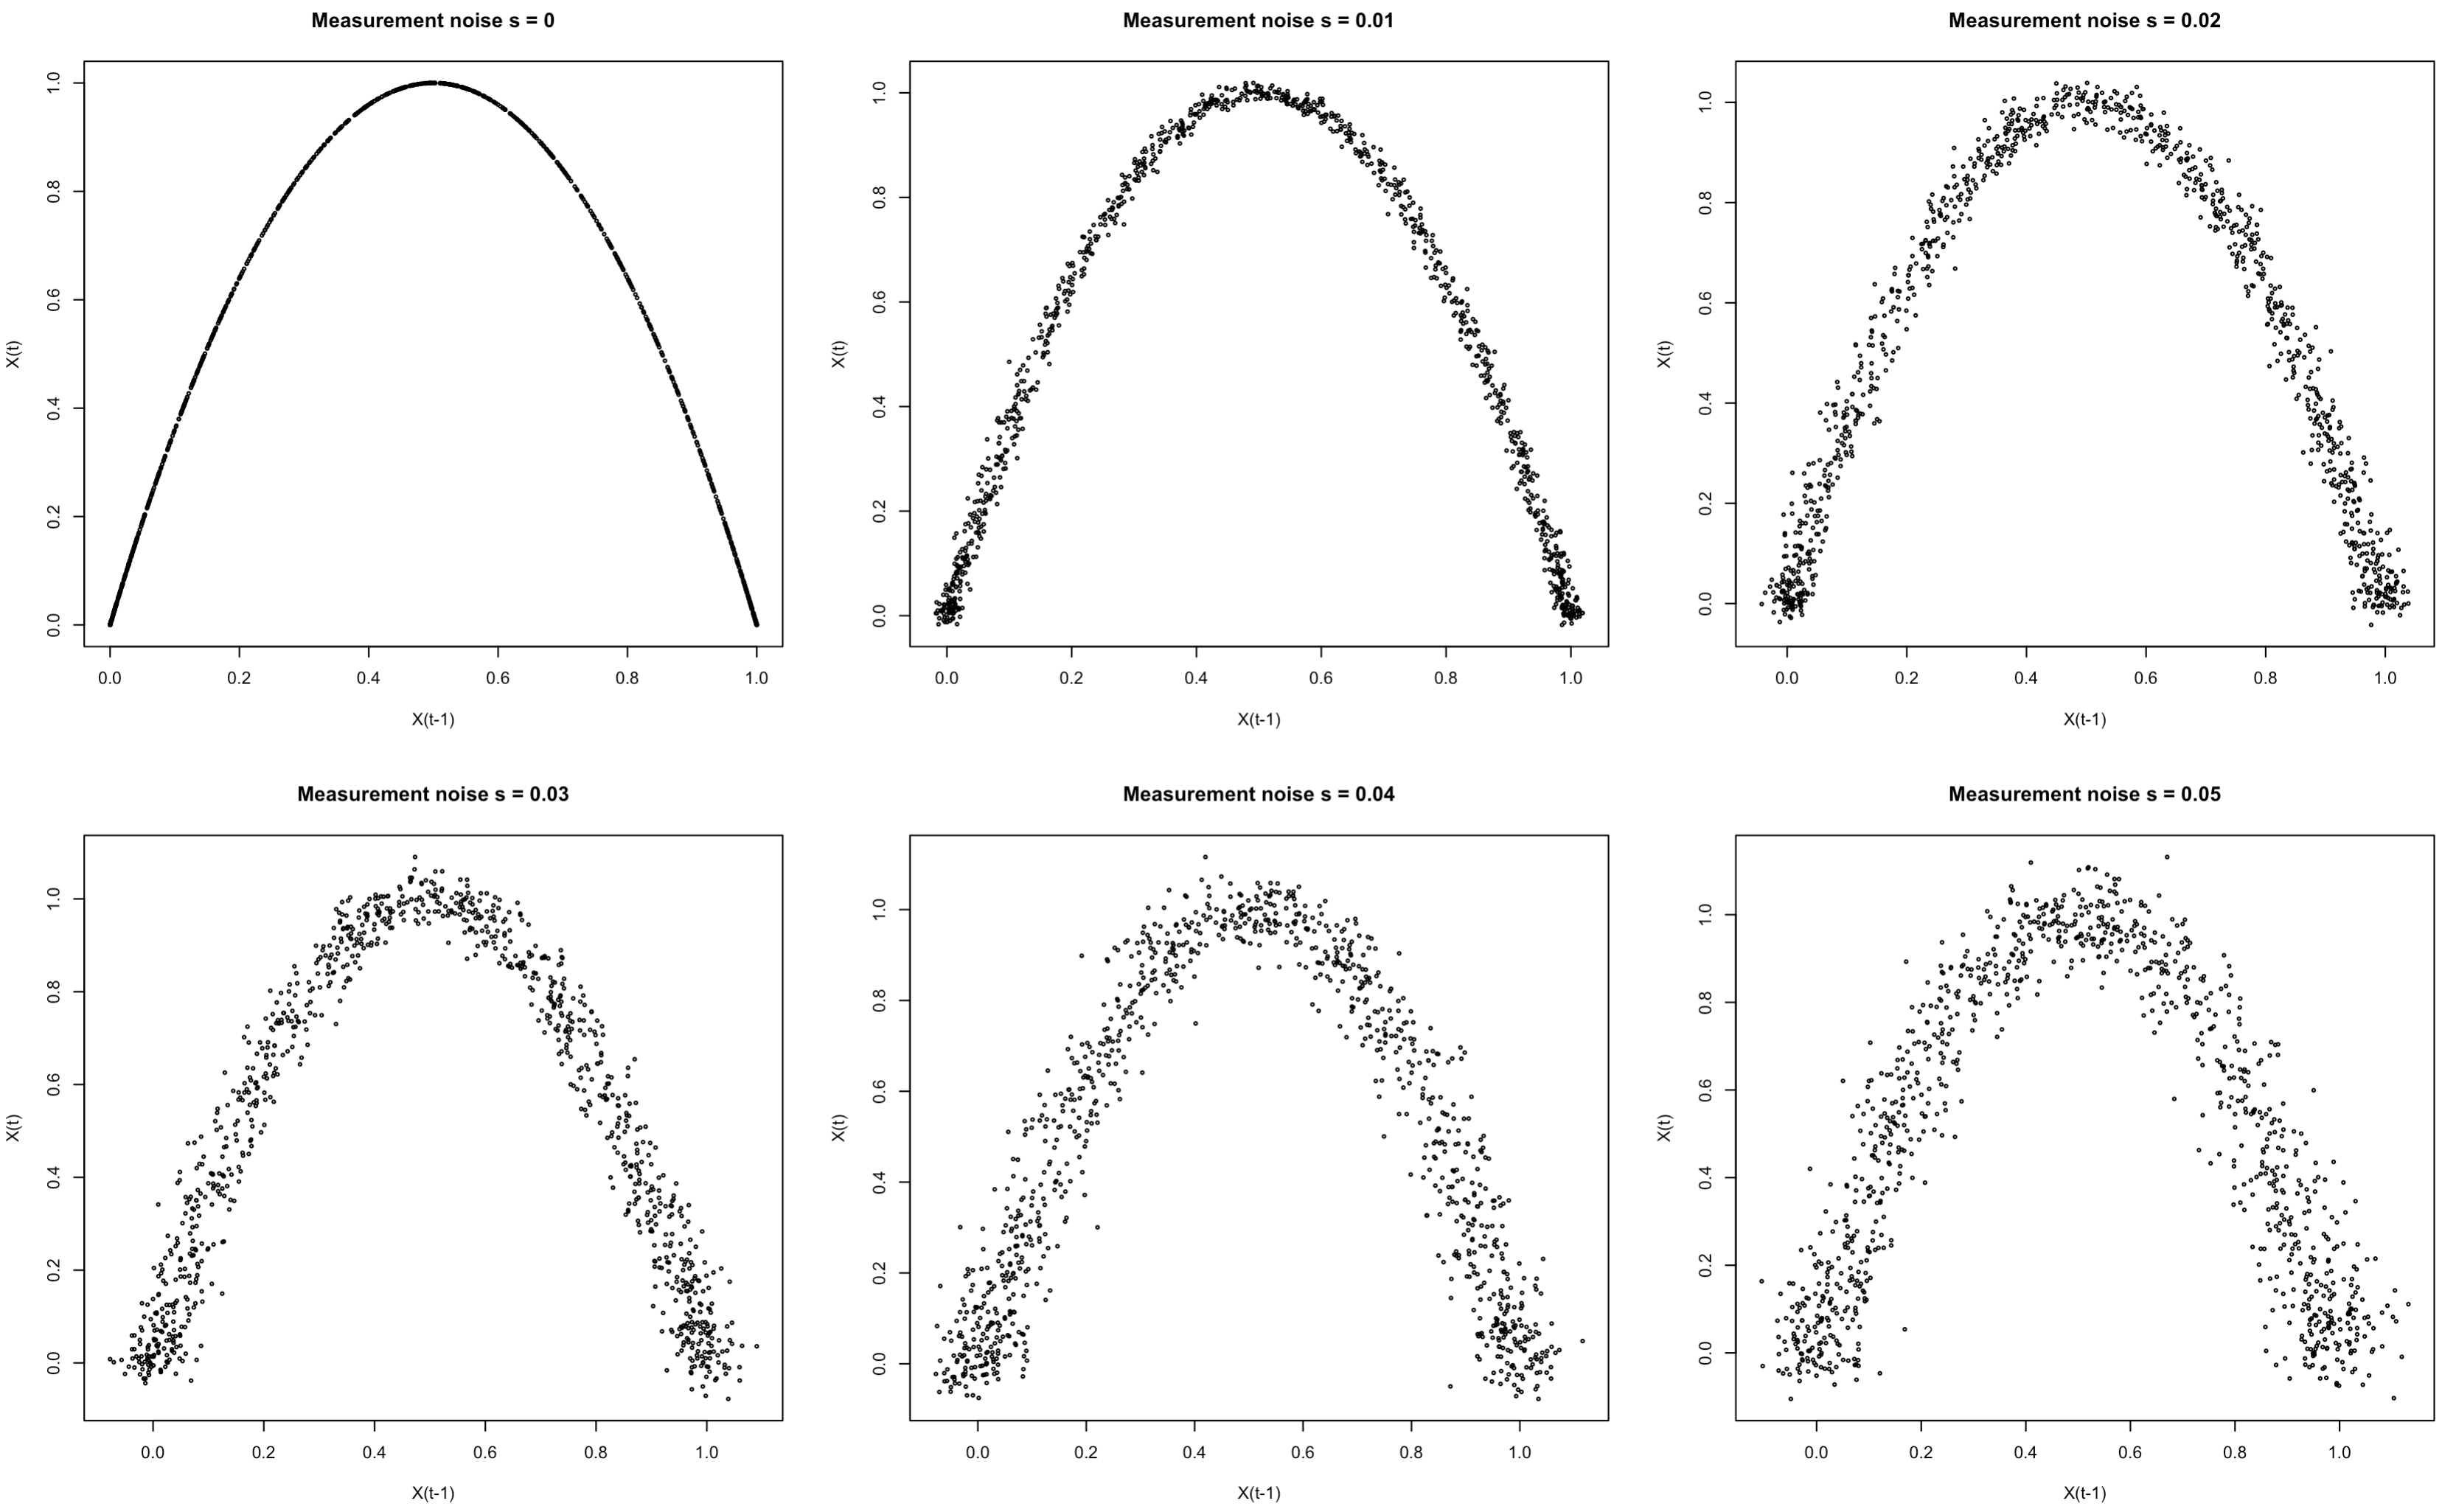
\includegraphics[width=\linewidth]{figure1}
\caption{\label{fig:1} Logistic map attractor adding a measurement noise with several variance values}
\end{figure}

In order to test the robustness of the different methods available to estimate the Lyapunov exponent, we are going to compare the results provided by the \pkg{tseriesChaos} package and the \pkg{nonlinearTseries} package with those of the \pkg{DChaos} package taking into account different measurement noise levels. We have considered four well-known chaotic dynamic systems. These datasets are available on the \pkg{DChaos} library; see Table \ref{tab:3}. 

The commands \code{install.packages("DChaos")} and \code{library(DChaos)} will download, install, and load the \pkg{DChaos} package so it can be used. The command \code{set.seed(34)} also will set the seed for reproducibility. To save CPU time, we have set the embedding dimension $1 \leqslant m \leqslant 7$, the time delay $\tau = 1$, the number of nodes in the single hidden layer  $2 \leqslant h \leqslant 10$, and the length of all time series data is $n = 1000$. We have considered only the bootstrap blocking method, and the number of bootstrap iterations is $B = 1000$. In this case, 63 different neural nets models have been estimated from each of the 24000 simulated series in order to obtain the results shown in table \ref{tab:4}. 

Note that the neural net models are sorted from lowest to highest BIC values. Then each best-fitted neural net model (with a lower BIC value) is considered to estimate the 24000 largest Lyapunov exponents. The mean square error (MSE) is calculated between the theoretical value and the value estimated by several direct and indirect methods. To do that, we have used the Monte Carlo method. We have done 1000 repetitions by different initial conditions when simulating the time-series data from the four dynamic systems and six measurement noise levels considered. 

The MSE values based on the estimation of the largest Lyapunov exponent from the direct methods provided by the \pkg{tseriesChaos} and \pkg{nonlinearTseries} packages are denoted by D1 and D2, respectively. Those obtained by the Jacobian indirect methods through the \pkg{DChaos} library are denoted by N2 (\code{lyapunov.max}) and QR (\code{lyapunov.spec}) regarding the Norma-2 and QR decomposition procedures, respectively. The results shown in table \ref{tab:4} provide the following comments. 

First, we can remark that our algorithms are robust to the presence of (small) measurement errors because the results obtained are comparable to those which are noise-free. Although as the noise increases, the error committed increases, but it is not proportional in any case. Second, the indirect methods provide better estimates than direct methods in all the experiments we have conducted. The algorithms proposed by the \pkg{tseriesChaos} package behave better than those of the \pkg{nonlinearTseries} library. Between the two methods available in the \pkg{DChaos} package, we do not observe significant differences. 

\begin{table}[ht!]
\centering
\begin{adjustbox}{width=\textwidth}
\begin{tabular}{lllcc}
\hline 
Dynamic system & Equations                                                & Parameters      & ${\lambda _{th}}$ \\ \hline
Logistic         & ${x_t} = \mu{x_{t - 1}}\left( {1 - {x_{t - 1}}} \right)$ & $\mu  = 4$ & 0.69314 \\ \hline
Gauss         & ${x_t} = {e^{ - \alpha x_{t - 1}^2}} + \beta$ & $\alpha  = 6.2, \beta = -0.5$ & 0.38367 \\ \hline
H\'enon          & ${x_t} = 1 - ax_{t - 1}^2 + {y_{t - 1}}$                 & $a=1.4$ & 0.41921 \\
                 & ${y_t} = b{x_{t - 1}}$                                   & $b=0.3$ &-1.63479 \\ \hline
R\"ossler        & $\dot x =  - y - z \hfill$                               & $a=0.2$ & 0.07143 \\
                 & $\dot y = x + ay \hfill$                                 & $b=0.2$ & 0.00000 \\
                 & $\dot z = b + \left( {x - c} \right)z$                   & $c=5.7$ & -0.53943 \\ \hline
\end{tabular}
\end{adjustbox}
\caption{\label{tab:3} Theoretical Lyapunov exponents (${\lambda _{th}}$) from time-series data available on \pkg{DChaos} package.}
\end{table}

\begin{table}[ht!]
\centering
\begin{adjustbox}{width=\textwidth}
\begin{tabular}{l|cccccc}
\hline 
Logistic map&  $s=0$      & $s=0.01$  & $s=0.02$  & $s=0.03$      & $s=0.04$  & $s=0.05$  \\ \hline 
D1 direct method        & 0.0001220 & 0.0056643 & 0.0030120 & 0.003006 & 0.0033485 & 0.0030913 \\ 
D2 direct method          & 0.4802315 & 0.4765133 & 0.4814125 & 0.4815446 & 0.4790305 & 0.4830895\\ 
N2 indirect method      & 0.0000324 & 0.0000382 & 0.0000691 & 0.0000994 & 0.0001314 & 0.0001532 \\ 
QR indirect method       & 0.0000331 & 0.0000348 & 0.0000672 & 0.0000986 & 0.0000997 & 0.0001124 \\  \hline
Gauss map&        &   &   &       &   &   \\ \hline 
D1 direct method        & 0.0015270 & 0.0111180 & 0.0205349 & 0.0293853 & 0.0275621 & 0.0336681 \\ 
D2 direct method        & 0.1474216 & 0.1480353 & 0.1477251 & 0.1464405 & 0.1481204 & 0.1476371\\ 
N2 indirect method      & 0.0000436 & 0.0000526 & 0.0000555 & 0.0000678 & 0.0000719 & 0.0000944 \\ 
QR indirect method      & 0.0000618 & 0.0000656 & 0.0000672 & 0.0000782 & 0.0000817 & 0.0000924 \\  \hline
H\'enon  system&        &   &   &       &   &   \\ \hline 
D1 direct method        & 0.0035650 & 0.0067221 & 0.0092761 & 0.0100339 & 0.0141379 & 0.0189926 \\ 
D2 direct method        & 0.3121588 & 0.3133259 & 0.3145991 & 0.3115671 & 0.3226997 & 0.3178221\\ 
N2 indirect method      & 0.0000365 & 0.0000486 & 0.0000635 & 0.0000761 & 0.0000899 & 0.0000917 \\ 
QR indirect method      & 0.0000318 & 0.0000451 & 0.0000589 & 0.0000601 & 0.0000866 & 0.0000932 \\ \hline
R\"ossler  system&        &   &   &       &   &   \\ \hline 
D1 direct method        & 0.0024471& 0.0049521 & 0.0063189 & 0.0072719 & 0.0127326 & 0.0174911 \\ 
D2 direct method        & 0.6398841 & 0.6412752 & 0.6388524 & 0.6396631 & 0.6451333 & 0.6499127\\ 
N2 indirect method      & 0.0002477 & 0.0003529 & 0.0005997 & 0.0006122 & 0.0009521 & 0.0019947 \\ 
QR indirect method      & 0.0003168 & 0.0004891 & 0.0006070 & 0.0007155 & 0.0008190 & 0.0009268 \\  \hline
\end{tabular}
\end{adjustbox}
\caption{\label{tab:4} The mean square error (MSE) values based on the estimation of the largest Lyapunov exponent from direct methods provided by the \pkg{tseriesChaos} (D1) and \pkg{nonlinearTseries} (D2) packages are showed. Also, those obtained by the Jacobian indirect methods through the \pkg{DChaos} library are presented (N2 for \code{lyapunov.max} and QR for \code{lyapunov.spec}).}
\end{table}

\newpage
\noindent Third, the direct methods are surely less flexible and robust but much faster and still informative. The Jacobian indirect methods based on the neural net approach seems to perform well for every noisy time series data. The price we have to pay is a greater computational complexity from two points of view, the computing time and the tuning parameters (node weights). Fourth, we have only focused on the largest Lyapunov exponent as direct methods do not estimate the full spectrum. In addition, those methods do not allow us to make inferences about it. In our case, we will be able to do so. Hence, we are going to focus on the reliability of the proposed methods. We want to know the power and size of our algorithms.

Finally, we will focus on testing the reliability of the algorithms provided by the \pkg{DChaos} package. For this purpose, we have calculated the so-called size and power of our hypothesis test. Due to the test is based on probabilities, there is always a chance of making an incorrect conclusion. When one does a hypothesis test, two types of errors are possible. As a reminder, when the null hypothesis is true, and we reject it, we make a type I error. The probability of making a type I error is denoted by $\alpha$, which is the significance level that we set for our hypothesis test. An $\alpha$ of $0.05$ indicates that we are willing to accept a $5\%$ chance that we are wrong when we reject the null hypothesis. To lower this risk, we must use a lower value for $\alpha$. However, using a lower value for alpha means that we will be less likely to detect a true difference if one really exists. The probability of not rejecting the null hypothesis when it is true (not committing a type I error) is called the size of the test. When the null hypothesis is false, and we fail to reject it, we make a type II error. The probability of making a type II error is called beta, and is often denoted by $\beta$. We can decrease our risk of committing a type II error by ensuring our test has enough power. We can do this by ensuring our sample size is large enough to detect a practical difference when one truly exists. The probability of rejecting the null hypothesis when it is false (not committing a type II error) is called the power of the test.

In order to understand the interrelationship between the type error I and II, in this case, consider the following. As we pointed out before, feasible test statistics were introduced, and a one-sided test was proposed for the purpose of testing the hypothesis of chaos (eq.\ref{eq0}) based on the theoretical asymptotic properties of the neural net estimator. Under the null hypothesis $H_0$ that the data-generating process is chaotic, the neural net estimator ${{\hat \lambda }_k}$ leads to asymptotically valid inferences in that the associated $p$-value follows a normal distribution on $N\left( {0,{{\hat \varphi }_k}} \right)$. Hence, our interest will be to test the null hypothesis ${H_0}:{{\hat \lambda }_k} > 0$ against the alternative ${H_1}:{{\hat \lambda }_k} \leqslant 0$. We will reject the null hypothesis if ${{\hat t}_k} \leqslant  - {z_\alpha }$, where ${{z_\alpha }}$ is the critical value that satisfies $\Pr \left[ {Z \geqslant {z_\alpha }} \right] = \alpha$ with $Z$ being a standard normal random variable and $\alpha$ is the significance level. Rejecting the null hypothesis ${H_0}:{{\hat \lambda }_k} > 0$ means lack of chaotic behavior. That is, the data-generating process does not have a chaotic attractor because it does not show the property of sensitivity to initial conditions. Thus, we have used these results to calculate the standard error of the Lyapunov exponent estimator and investigate the statistical significance of the sign of the exponents in order to test the reliability of the proposed algorithms.

\begin{table}[ht!]
\centering
\begin{adjustbox}{width=\textwidth}
\begin{tabular}{l|cccccc}
\hline 
$n=50$ &  $s=0$      & $s=0.01$  & $s=0.02$  & $s=0.03$      & $s=0.04$  & $s=0.05$  \\ \hline
Logistic map    & 2.40 & 2.60 & 3.60 & 3.50 & 3.30 & 4.10 \\ 
Gauss map          & 2.70 & 3.60 & 4.20 & 4.70 & 4.30 & 4.70\\ 
H\'enon  system   & 2.90 & 3.70 & 3.90 & 4.00 & 4.50 & 4.30\\ 
R\"ossler  system       & 3.10 & 3.50 & 4.70 & 4.90 & 4.50 & 5.10\\ \hline
$n=100$ &        &   &   &       &   &   \\ \hline
Logistic map        & 1.20 & 1.50 & 2.30 & 2.50 & 3.40 & 3.90\\ 
Gauss map             & 1.50 & 1.70 & 1.90 & 2.70 & 3.10 & 3.50\\ 
H\'enon  system      & 1.70 & 1.90 & 2.20 & 3.30 & 3.70 & 4.00\\
R\"ossler  system        & 1.70 & 1.80 & 2.30 & 4.10 & 3.70 & 4.70\\ \hline
$n=200$ &        &   &   &       &   &   \\ \hline
Logistic map       & 0.30 & 0.50 & 1.20 & 1.40 & 1.50 & 2.10\\ 
Gauss map            & 0.50 & 0.80 & 0.90 & 1.10 & 1.40 & 2.50\\ 
H\'enon  system     & 0.40 & 0.60 & 0.70 & 1.80 & 1.90 & 2.20\\ 
R\"ossler  system       & 0.50 & 1.10 & 1.30 & 1.70 & 2.50 & 3.30\\ \hline
\end{tabular}
\end{adjustbox}
\caption{\label{tab:5} Rejection percentages at the $5\%$ significance level from the dynamic systems considered with a chaotic behaviour. These results provide the size of our hypothesis test.}
\end{table}
\newpage
Note that the results shown in tables \ref{tab:5}-\ref{tab:6} are given in terms of rejection percentages of the tests at the $5\%$ significance level over 1000 Monte Carlo replications. The rejection percentages give an indication of the size of the tests (tab.\ref{tab:5}) and the power of the tests (tab.\ref{tab:6}). We have chosen $n=50, 100, 200$ as we want to check the reliability of the algorithms in small sample sizes. The four dynamic systems used are listed in tab.\ref{tab:3}. Table \ref{tab:5} provides the results from chaotic dynamic systems which have the following parameter set values: $\mu=4$ (logistic map); $\alpha=6.2, \beta=-0.5$ (Gauss map); $a=1.4, b=0.3$ (H\'enon system), and $a=0.2, b=0.2, c=5.7$ (R\"ossler system). Table \ref{tab:6} gives the results from non-chaotic dynamic systems which have the following parameter set values: $\mu=3.2$ (logistic map); $\alpha=4.9, \beta=-0.58$ (Gauss map); $a=1.2, b=0.1$ (H\'enon system), and $a=0.1, b=0.1, c=7$ (R\"ossler system).

The data given in tables \ref{tab:5}-\ref{tab:6} provide the following comments. First, we can point out that the reliability of the tests is solid at the $5\%$ significance level. The rejection percentages in almost every situation, even for $n=50$, are low when the null hypothesis ${H_0}$ is true and high when ${H_0}$ is false. Second, the results provide satisfactory performance in moderate sample sizes. This fact is really important for those researchers who work with short time series data. Third, the empirical size decrease and the empirical power increase as the sample size increase which means that our tests are consistent as well. Fourth, the noise-contaminated data are comparable to those which are noise-free. Although as the noise increases, the errors committed increase but not significantly. Fifth, the results shown are fairly robust with respect to the parameter values of the four dynamic systems considered. 

\begin{table}[ht!]
\centering
\begin{adjustbox}{width=\textwidth}
\begin{tabular}{l|cccccc}
\hline 
$n=50$ &  $s=0$      & $s=0.01$  & $s=0.02$  & $s=0.03$      & $s=0.04$  & $s=0.05$  \\ \hline
Logistic map        & 99.30 & 98.90 & 98.40 & 97.70 & 97.50 & 96.90 \\ 
Gauss map          & 99.40 & 99.00 & 98.70 & 98.50 & 97.10 & 97.00\\ 
H\'enon  system      & 99.20 & 98.90 & 98.60 & 97.90 & 97.40 & 96.90\\ 
R\"ossler  system        & 98.70 & 98.10 & 97.40 & 97.00 & 96.70 & 96.20\\ \hline
$n=100$ &        &   &   &       &   &   \\ \hline
Logistic map        & 99.70 & 99.00 & 98.70 & 98.20 & 97.70 & 97.20\\ 
Gauss map          & 99.70 & 99.30 & 98.90 & 98.70 & 98.40 & 97.70\\ 
H\'enon  system      & 99.60 & 99.00 & 98.80 & 98.20 & 97.70 & 97.10\\
R\"ossler  system        & 99.40 & 98.80 & 98.30 & 97.70 & 97.20 & 96.90\\ \hline
$n=200$ &        &   &   &       &   &   \\ \hline
Logistic map        & 99.90 & 99.40 & 99.00 & 98.70 & 98.20 & 97.90\\ 
Gauss map           & 100.00 & 99.60 & 99.30 & 99.00 & 98.80 & 98.20\\ 
H\'enon  system      & 99.80 & 99.30 & 99.00 & 98.60 & 98.10 & 97.80\\ 
R\"ossler  system        & 99.70 & 99.00 & 98.70 & 98.20 & 97.50 & 97.00\\ \hline
\end{tabular}
\end{adjustbox}
\caption{\label{tab:6} Rejection percentages at the $5\%$ significance level from the dynamic systems considered with a non-chaotic behaviour. These results provide the power of our hypothesis test.} 
\end{table}

%%%%%%%%%%%%%%%%%%%%%%%%%%%%%%%%
%%%%%%%%%%%% CONCLUSION %%%%%%%%%%%%
%%%%%%%%%%%%%%%%%%%%%%%%%%%%%%%%

\section{Conclusion}

The main feature of chaos is the well-known initial-value sensitivity property. The study of measures to quantify the initial-value sensitive property began with the introduction of Lyapunov exponents. So quantifying chaos through this kind of quantitative measure is a key point for understanding chaotic behavior. This paper describes the main statistical estimation methods of the Lyapunov exponent from time series data. At the same time, we present the \pkg{DChaos} library. This package provides an R interface for chaotic time series data analysis. R itself and all packages used are available from the Comprehensive R Archive Network (CRAN) at \url{https://CRAN.R-project.org/}.

 R users may compute the delayed-coordinate embedding vectors from time series data, estimates the best neural net model, calculates the partial derivatives directly from the chosen neural network model. Finally, they can estimate both the largest Lyapunov exponent through the Norma-2 procedure and the Lyapunov exponent spectrum through the QR decomposition procedure taking into account the full sample and three different methods of subsampling by blocks. The results provided by \cite{Shintani2004} have enabled us to obtain a consistent Lyapunov exponent estimator and test the chaotic hypothesis based on the theoretical asymptotic properties of our neural net estimators.

Finally, looking to the future, our focus will be on extending the functionality of this package. Let us remark that the different contributions that compose the Jacobian indirect methods differ in the algorithm used for the estimation of the Jacobian. So far, we have focused on the neural net approach, which tries to estimate the underlying dynamic system without imposing the restriction of local linearity. We are working on three more Jacobian indirect methods that try to estimate the Jacobian by local polynomial kernel regressions, by local neural nets models, and by convolutional neural nets models. We are interested in developing the proposed algorithms from multivariate time series data. We are also focusing on how to apply parallelization and big data techniques to the design of the proposed algorithms in order to obtain computational efficiency when applying them to massive databases. We will keep providing useful tools and robust algorithms related to the analysis of chaotic time-series data.

%%%%%%%%%%%%%%%%%%%%%%%%%%%%%%%%
%%%%%%%%%% ACKNOWLEDGMENTS %%%%%%%%%
%%%%%%%%%%%%%%%%%%%%%%%%%%%%%%%%

\section{Acknowledgment}

This work was supported by the Government of Spain (grant RTI2018-094901-B-I00); the Complutense University of Madrid (Faculty of Statistical Studies); the San Pablo CEU University (Faculty of Economics); and the Data Analysis in Social and Gender Studies and Equality Policies Research Group (\url{www.ucm.es/aedipi/}). 

%%%%%%%%%%%%%%%%%%%%%%%%%%%%%%%%
%%%%%%%%%% BIBLIOGRAPHY %%%%%%%%%%%%%
%%%%%%%%%%%%%%%%%%%%%%%%%%%%%%%%

\bibliography{sandubete-escot}

\address{Julio E. Sandubete\\
  Faculty of Statistical Studies\\
  Complutense University of Madrid\\
  28040 Madrid, Spain\\
  ORCiD: 0000-0002-1518-0417\\
  E-mail:} \email{jsandube@ucm.es} \\

\address{Lorenzo Escot\\
  Faculty of Statistical Studies\\
  Complutense University of Madrid\\
  28040 Madrid, Spain\\
  ORCiD: 0000-0002-6734-6327\\
E-mail:} \email{escot@ucm.es}

